\documentclass[10pt,a4paper]{article}
\usepackage[UTF8]{ctex}
\setCJKmainfont[BoldFont=黑体,ItalicFont=楷体]{华文中宋}
\usepackage{amssymb,amsmath,amsfonts,amsthm,mathrsfs,dsfont,graphicx}
\usepackage{ifthen,indentfirst,enumerate,color,titletoc}
\usepackage{tikz}
\usepackage{multicol}
\usepackage{makecell}
\usepackage{longtable}
\usepackage{ifthen}
\usetikzlibrary{arrows,calc,intersections,patterns,decorations.pathreplacing,3d,angles,quotes}
\usepackage[bf,small,indentafter,pagestyles]{titlesec}
\usepackage[top=1in, bottom=1in,left=0.8in,right=0.8in]{geometry}
\renewcommand{\baselinestretch}{2}
\newtheorem{defi}{定义~}
\newtheorem{eg}{例~}
\newtheorem{ex}{~}
\newtheorem{rem}{注~}
\newtheorem{thm}{定理~}
\newtheorem{coro}{推论~}
\newtheorem{axiom}{公理~}
\newtheorem{prop}{性质~}
\newcommand{\blank}[1]{\underline{\hbox to #1pt{}}}
\newcommand{\bracket}[1]{(\hbox to #1pt{})}
\newcommand{\onech}[4]{\par\begin{tabular}{p{.9\textwidth}}
A.~#1\\
B.~#2\\
C.~#3\\
D.~#4
\end{tabular}}
\newcommand{\twoch}[4]{\par\begin{tabular}{p{.46\textwidth}p{.46\textwidth}}
A.~#1& B.~#2\\
C.~#3& D.~#4
\end{tabular}}
\newcommand{\vartwoch}[4]{\par\begin{tabular}{p{.46\textwidth}p{.46\textwidth}}
(1)~#1& (2)~#2\\
(3)~#3& (4)~#4
\end{tabular}}
\newcommand{\fourch}[4]{\par\begin{tabular}{p{.23\textwidth}p{.23\textwidth}p{.23\textwidth}p{.23\textwidth}}
A.~#1 &B.~#2& C.~#3& D.~#4
\end{tabular}}
\newcommand{\varfourch}[4]{\par\begin{tabular}{p{.23\textwidth}p{.23\textwidth}p{.23\textwidth}p{.23\textwidth}}
(1)~#1 &(2)~#2& (3)~#3& (4)~#4
\end{tabular}}
\begin{document}

\begin{enumerate}[1.]

\item 自由落体运动的位移$d$(单位: $\text{m}$)与时间$t$(单位: $\text{s}$)满足函数关系$d=\dfrac 12gt^2$($g$为重力加速度).\\
(1) 分别求$[4,4.1]$、$[4,4.01]$、$[4,4.001]$这些时间段内自由落体的平均速度;\\
(2) 求$t=4$时的瞬时速度;\\
(3) 求$t=a$($a>0$)时的瞬时速度;\\
(4) 借助(3)的结果, 求$t=\dfrac 52$时的瞬时速度.
\item 竖直向上发射的火箭熄火时上升速度达到$100\text{m}/\text{s}$, 此后其位移$H$(单位: $\text{m}$)与时间$t$(单位: $\text{s}$)近似满足函数关系$H=100t-5t^2$.\\
(1) 分别求火箭在$[0, 2]$、$[2, 4]$这些时间段内的平均速度;\\
(2) 求火箭在$t=2$时的瞬时速度;\\
(3) 熄火后多长时间火箭上升速度为$0$?
\item 某水管的流水量$y$(单位: $\text{m}^3$)与时间$t$(单位: $\text{s}$)满足函数关系$y=f(t)$, 其中$f(t)=3t$.\\
(1) 求$f(t)$在$t=a$处的导数$f'(a)$;\\
(2) $f'(a)$的实际意义是什么?\\
(3) 随着$a$的取值变化, $f'(a)$是否发生变化? 为什么?
\item 将石子投入水中, 水面产生的圆形波纹不断扩散. 计算:\\
(1) 当半径$r$从$a$增加到$a+h$($h>0$)时, 圆面积相对于半径的平均变化率;\\
(2) 当半径$r=a$时, 圆面积相对于半径的瞬时变化率. 
\item 函数$y=f(x)$的图像如图所示.
\begin{center}
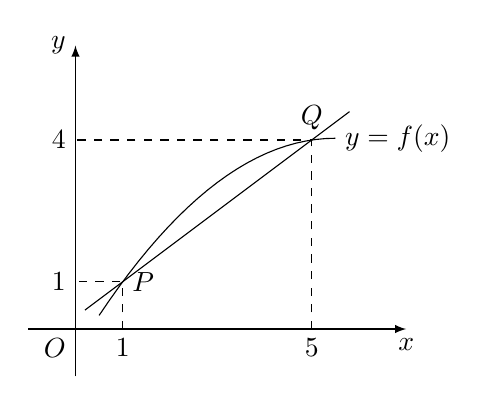
\begin{tikzpicture}[>=latex,scale = 0.6]
\draw [->] (-1,0) -- (7,0) node [below] {$x$};
\draw [->] (0,-1) -- (0,6) node [left] {$y$};
\draw (0,0) node [below left] {$O$};
\draw [dashed] (5,0) -- (5,4) coordinate (S) node [above] {$Q$} -- (0,4) (1,0) -- (1,1) coordinate (T) node [right] {$P$} -- (0,1);
\draw (1,0) node [below] {$1$} (5,0) node [below] {$5$} (0,1) node [left] {$1$} (0,4) node [left] {$4$};
\draw ($(S)!-0.2!(T)$) -- ($(T)!-0.2!(S)$);
\draw [domain = 0.5:5.5] plot (\x,{-(1/2)+(33*\x)/20-3*pow(\x,2)/20}) node [right] {$y=f(x)$};
\end{tikzpicture}
\end{center}
(1) 求割线$PQ$的斜率;\\
(2) 当点$Q$沿曲线向点$P$运动时, 割线$PQ$的斜率会变大还是变小? 
\item 已知$f(x)=-x^2$, 求曲线$y=f(x)$在下列各点处的切线斜率, 并说明这些斜率的值是如何随着自变量的变化而变化的:
(1) $x=-2$;\\
(2) $x=-1$;\\
(3) $x=0$;\\
(4) $x=1$;\\
(5) $x=2$.
\item 借助函数图像, 判断下列导数的正负:\\
(1) $f'(-\dfrac \pi 4)$, 其中$f(x)=\cos x$;\\
(2) $f'(3)$, 其中$f(x)=\ln x$.
\item 已知车辆启动后的一段时间内, 车轮旋转的角度和时间(单位: 秒)的平方成正比, 且车辆启动后车轮转动第一圈需要$1$秒.\\
(1) 求车轮转动前$2$秒的平均角速度;\\
(2) 求车轮在转动开始后第$3$秒的瞬时角速度.
\item 根据导数的几何意义, 求函数$y=\sqrt{4-x^2}$在下列各点处的导数:\\
(1) $x=-1$;\\
(2) $x=0$;\\
(3) $x=1$.
\item 已知函数$y=f(x)$在$x=1$处的切线方程为$y=4x-3$, 求$f(1)$和$f'(1)$.
\item 如图, 已知直线$l$是曲线$y=f(x)$在$x=3$处的切线, 求$f'(3)$.
\begin{center}
\begin{tikzpicture}[>=latex,scale = 0.6]
\draw [->] (-5,0) -- (5,0) node [below] {$x$};
\draw [->] (0,-3) -- (0,3) node [left] {$y$};
\draw (0,0) node [below left] {$O$};
\draw (-5,-1) .. controls (0,4) and (0,-1) .. (3,-2);
\draw (3,-2) .. controls (3.9,-2.3) and (4,-1).. (5,-1) node [right] {$y=f(x)$};
\filldraw (0,-1) circle (0.05) node [below left] {$-1$} coordinate (Q);
\filldraw (3,-2) circle (0.05) node [below] {$P$} coordinate (P);
\draw ($(P)!-1!(Q)$) node [right] {$l$} -- ($(P)!2.5!(Q)$);
\draw [dashed] (3,0) node [below right] {$3$} -- (3,-2) -- (0,-2) node [left] {$-2$};
\end{tikzpicture}
\end{center}
\item 求下列函数$y=f(x)$的导数:\\
(1) $f(x)=\pi$;\\
(2) $f(x)=\sqrt[3]{x^5}$;\\
(3) $f(x)=\dfrac1{x^3}$.
\item 求曲线$y=\cos x$在$x=\pi 2$处的切线方程.
\item 已知曲线$y=x^3$在原点以外某点$P$处切线的斜率为$a$.\\
(1) 求点$P$的坐标;\\
(2) 判断$a$的正负.
\item 求曲线$y=x^3-3x+5$平行于$x$轴的切线及其切点坐标.
\item 求曲线$y=\dfrac 1x$平行于直线$y=-x$的切线及其切点坐标.
\item 求下列函数$y=f(x)$的导数:\\
(1) $f(x)=2x^{\mathrm{e}}-\mathrm{e}^2$;\\
(2) $f(x)=\mathrm{e}^x\cos x$;\\
(3) $f(x)=\dfrac{x-1}{x-2}$;\\
(4) $f(x)=\dfrac{\ln x}{\sin x}$.
\item 用两种方法求函数$y=(x-2)(3-4x)$的导数.
\item 已知函数$y=f(x)$与$y=g(x)$满足条件$f(1)=2$, $f'(1)=3$, $g(1)=4$与$g'(1)=5$.对于下列函数$y=h(x)$, 求$h(1)$和$h'(1)$:\\
(1) $h(x)=2g(x)-\dfrac 13f(x)$;\\
(2) $h(x)=2g(x)f(x)-\dfrac 13$;\\
(3) $h(x)=\dfrac{2g(x)-1}{3f(x)}$.
\item 利用$y=f(ax+b)$型复合函数的求导法则, 求下列函数的导数:\\
(1) $y= \sqrt{2x-5}$;\\
(2) $y=\cos \dfrac x2$;\\
(3) $y= \dfrac 1{\mathrm{e}^{x+1}}$.
\item 用两种方法求函数$y= \dfrac 2{x-1}$的导数.
\item 某种动物的体温犜(单位: $^\circ\text{C}$)与太阳落山后经过的时间$t$(单位: $\text{min}$)满足函数关系$T=\dfrac{120}{t+5}+15$.\\
(1) 当$t=5$时, 求该动物体温的瞬时变化率;\\
(2) 在哪一时刻该动物体温的瞬时变化率是$-2^\circ\text{C}/\text{min}$? (结果精确到$0.1\text{min}$)
\item 已知某港口一天内潮水的深度$y$(单位: $\text{m}$)与时间$t$(单位: $\text{h}$)近似满足函数关系$y=3\sin (\dfrac \pi {12}t+\dfrac{5\pi} 6)$, $0\le t\le 24$. 分别求上午$6$时与下午$6$时潮水涨(落)的速度.
\item 已知一列火车从静止开始加速的一段时间内, 其行驶速度$v$(单位: $\text{m}/\text{s}$)与行驶时间$t$(单位: $\text{s}$)满足函数关系$V=0.4t+0. 6t^2$.\\
(1) 求这段时间内火车行驶的加速度;\\
(2) 火车行驶到哪一时刻, 其加速度为$4\text{m}/\text{s}^2$?
\item 直线$y=-x+b$是下列函数的切线吗? 如果是, 请求出$b$的值; 如果不是, 请说明理由.\\
(1) $y=\ln x$;\\
(2) $y=\dfrac 1x$.
\item 吹一个球形的气球时, 气球半径$r$将随空气容量$V$的增加而增大.\\
(1) 写出气球半径$r$关于气球内空气容量$V$的函数表达式;\\
(2) 求$V=1$时, 气球的瞬时膨胀率(即气球半径关于气球内空气容量的瞬时变化率).
\item 判断下列求导结果是否正确. 如果不正确, 请指出错在哪里, 并予以改正.\\
(1) $(\dfrac{\sin x}x)'=-\dfrac 1{x^2}\sin x-\dfrac{\cos x}x$;\\
(2) $(\ln (2-x))'=\dfrac 1{2-x}$.
\item 求过点$(0, -1)$且与曲线$y=2x^2$相切的直线的方程.
\item 已知一罐汽水放入冰箱后的温度$x$(单位: $^\circ\text{C}$)与时间$t$(单位: $\text{h}$)满足函数关系$x=4+16\mathrm{e}^{-2t}$.\\
(1) 求$x'(1)$, 并解释其实际意义;\\
(2) 已知摄氏度$x$与华氏度$y$(单位: $^\circ\text{F}$)满足函数关系$x=\dfrac 59(y-32)$, 求$y$关于$t$的导数, 并解释其实际意义.
\item 求下列函数$y=f(x)$的导数, 其中:\\
(1) $f(x)=x^2\sin 3x-\dfrac 2{\sqrt x}$;\\
(2) $f(x)=\dfrac{\mathrm{e}^x-\mathrm{e}^{-x}}{\mathrm{e}^x+\mathrm{e}^{-x}}$.
\item 利用导数研究下列函数的单调性, 并说明结果与你之前的认识是否一致:\\
(1) $y=(\dfrac 1{\mathrm{e}})^x$;\\
(2) $y=\log_{\frac 1{\mathrm{e}}}x$.
\item 利用导数判断函数$y= \dfrac 1{\cos x}$, $x\in (-\dfrac\pi 2, \dfrac \pi 2)$的单调性, 并求出极值.
\item 某函数图像如图所示, 它在$[a, b]$上哪一点处取得最大值? 它是极大值点吗? 在哪一点处取得最小值? 它是极小值点吗? 
\begin{center}
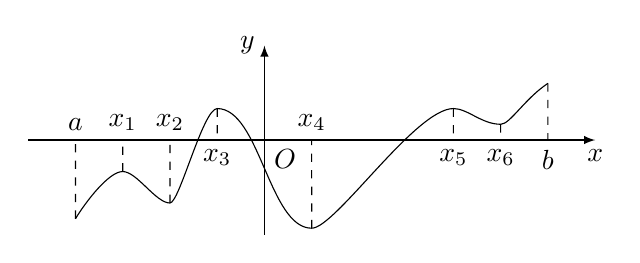
\begin{tikzpicture}[>=latex,xscale = 0.6,yscale = 0.4]
\draw [->] (-5,0) -- (7,0) node [below] {$x$};
\draw [->] (0,-3) -- (0,3) node [left] {$y$};
\draw (0,0) node [below right] {$O$};
\draw (-4,-2.5) coordinate (A) .. controls (-3.8,-2) and (-3.3,-1) .. (-3,-1) coordinate (B) .. controls (-2.7,-1) and (-2.3,-2) .. (-2,-2) coordinate (C) .. controls (-1.8,-2) and (-1.3,1) .. (-1,1) coordinate (D) .. controls (-0.1,1) and (0.1,-2.8) .. (1,-2.8) coordinate (E) .. controls (1.5,-2.8) and (3.2,1) .. (4,1) coordinate (F) .. controls (4.3,1) and (4.6,0.5) .. (5,0.5) coordinate (G) .. controls (5.2,0.5) and (5.5,1.3) .. (6,1.8) coordinate (H);
\draw [dashed] (A) -- (-4,0) node [above] {$a$} (B) -- (-3,0) node [above] {$x_1$} (C) -- (-2,0) node [above] {$x_2$} (D) -- (-1,0) node [below] {$x_3$} (E) -- (1,0) node [above] {$x_4$} (F) -- (4,0) node [below] {$x_5$} (G) -- (5,0) node [below] {$x_6$} (H) -- (6,0) node [below] {$b$};
\end{tikzpicture}
\end{center}
\item 求下列函数的单调区间、极值点和极值:\\
(1) $y=x^2+2x+3$;\\
(2) $y=x+\dfrac 1x$;\\
(3) $y=3x-x^3$;\\
(4) $y=x^2\mathrm{e}^x$.
\item 证明:函数$y=x^3+4x$在$(-\infty, +\infty)$上严格增.
\item 求函数$y=-x^3+12x-1$的单调减区间.
\item 证明:函数$y=x-\dfrac 1x$没有极值点.
\item 求函数$y=-x^3+12x-1$, $x\in [0, 3]$的值域.
\item 判断下列函数在$(-\infty, +\infty)$上是否存在驻点, 是否存在极值点, 并说明理由:\\
(1) $y=x^n$, $n$为正奇数;\\
(2) $y=x^n$, $n$为正偶数.
\item 已知函数$y=x^3+2mx^2-nx+m$在$x=1$处有极值$0$, 求$m+n$的值.
\item 用长为$18\text{m}$的钢条制作一个如图所示的长方体框架. 已知长方体的长宽比为$2:1$, 问:该长方体的长、宽、高各为多少时, 其体积最大? 最大体积是多少?
\begin{center}
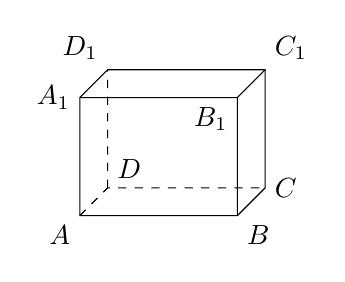
\begin{tikzpicture}[>=latex]
\draw (0,0) node [below left] {$A$} coordinate (A) --++ (2,0) node [below right] {$B$} coordinate (B) --++ (45:{1/2}) node [right] {$C$} coordinate (C)
--++ (0,1.5) node [above right] {$C_1$} coordinate (C1)
--++ (-2,0) node [above left] {$D_1$} coordinate (D1) --++ (225:{1/2}) node [left] {$A_1$} coordinate (A1) -- cycle;
\draw (A) ++ (2,1.5) node [below left] {$B_1$} coordinate (B1) -- (B) (B1) --++ (45:{1/2}) (B1) --++ (-2,0);
\draw [dashed] (A) --++ (45:{1/2}) node [above right] {$D$} coordinate (D) --++ (2,0) (D) --++ (0,1.5);
\end{tikzpicture}
\end{center}
\item 某分公司经销一品牌产品, 每件产品的成本为$4$元, 且每件产品需向总公司交$3$元的管理费, 预计当每件产品的售价为$x$元($8\le x\le 11$)时, 一年的销售量为$(12-x)^2$万件. 问:当每件产品的售价为多少元时, 该分公司一年的利润犔最大? (结果精确到$1$元)
\item $4$名学生分别报名参加学校的足球队、篮球队和棒球队, 每人限报其中的一支. 问: 有多少种不同的报名方法? 
\item 某服装厂为学校设计了$4$种样式的上衣、$3$种样式的裤子. 若取其中的一件上衣和一条裤子配成校服, 则可以配出多少种不同样式的校服? 
\item 在一种编码方式中, 每个编码都是两位字符, 规定第一位用数字$0$至$9$中之一, 第二位用$26$个小写英文字母中之一. 这种编码方式共可以产生多少个不同的编码? 
\item 设集合$A=\{(x, y)|x\in \mathbf{Z}, \  y\in \mathbf{Z}, \  \text{且}|x|\le 6, \ |y|\le 7\}$, 则集合$A$中有多少个元素?
\item 从$a$、$b$、$c$、$d$、$e$这$5$个元素中取出$4$个, 放在$4$个不同的格子中, 且元素$b$不能放在第二个格子里. 问:一共有多少种不同的放法?
\item $A$、$B$、$C$、$D$、$E$五人站成一排, 如果$B$必须站在$A$的右边($A$、$B$可以不相邻), 那么有多少种不同的排法?
\item 乘积$(a_1+a_2)(b_1+b_2+b_3)(c_1+c_2+c_3+c_4)$的展开式中有多少项? 
\item 如图, 要接通从$A$到$B$的电路, 不同的接通方法有多少种?
\begin{center}
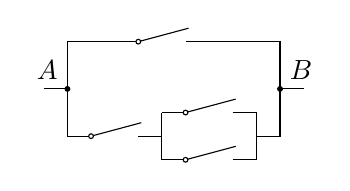
\begin{tikzpicture}[>=latex,scale = 0.6]
\draw (0,0) -- (0.5,0) (1.5,0) -- (2,0) (2,0.5) -- (2,-0.5) -- (2.5,-0.5) (2,0.5) -- (2.5,0.5) (3.5,0.5) -- (4,0.5) -- (4,-0.5) -- (3.5,-0.5) (4,0) -- (4.5,0) -- (4.5,2) -- (2.5,2) (1.5,2) -- (0,2) -- (0,0) (-0.5,1) -- (0,1) (4.5,1) -- (5,1);
\filldraw (0,1) circle (0.05) node [above left] {$A$} (4.5,1) circle (0.05) node [above right] {$B$};
\draw (0.5,0) --++ (15:1.1) (2.5,0.5) --++ (15:1.1) (2.5,-0.5) --++ (15:1.1) (1.5,2) --++ (15:1.1);
\filldraw [fill = white, draw = black] (0.5,0) circle (0.05) (2.5,0.5) circle (0.05) (2.5,-0.5) circle (0.05) (1.5,2) circle (0.05);
\end{tikzpicture}
\end{center}
\item 用$1$、$2$、$3$、$4$、$5$、$6$组成没有重复数字的六位数, 要求所有相邻两个数字的奇偶性都不同, 且$1$和$2$相邻. 问:有多少个这样的六位数? 
\item 已知$p_1$、$p_2$、$p_3$是互不相同的素数, $\alpha$、$\beta$、$\gamma$是正整数, $n=p_1^\alpha p_2^\beta p_3^\gamma$. 问: $n$有多少个不同的正约数?
\item 用$1$、$2$、$3$、$4$可以组成多少个没有重复数字的四位正整数?  其中有多少个偶数? 
\item 从$1$、$2$、$3$、$4$、$5$这$5$个数字中, 任取$2$个不同的数字作为一个点的坐标, 一共可以组成多少个不同的点? 
\item 在方程$ax+by=0$中, 设系数$a$、$b$是集合$\{0, 1, 2, 3, 5, 7\}$中两个不同的元素. 求这些方程所表示的不同直线的条数.
\item 将$5$个人排成一排, 若甲和乙必须排在一起, 则有多少种不同的排法? 
\item 从$7$名运动员中选$4$名组成接力队参加$4\times 100$米接力赛. 问:甲、乙两人都不跑中间两棒的排法有多少种? 
\item 从$7$名男生和$5$名女生中选取$3$人依次进行面试.\\
(1) 若参加面试的人全是女生, 则有多少种不同的面试方法?
(2) 若参加面试的人中, 恰好有$1$名女生, 则有多少种不同的面试方法? 
\item 若$m$为正整数, 且$m<27$, 则$(27-m)(28-m)\cdots(34-m)$等于\bracket{20}.
\fourch{$\mathrm{P}_{27-m}^8$}{$\mathrm{P}_{34-m}^{27-m}$}{$\mathrm{P}_{34-m}^7$}{$\mathrm{P}_{34-m}^8$}
\item 求满足等式$\mathrm{P}_{2n}^3=28\mathrm{P}_n^2$的正整数$n$的值.
\item 解关于正整数$x$的不等式$\mathrm{P}_8^x<6\mathrm{P}_8^{x-2}$.
\item 有$4$张分别标有数字$1$、$2$、$3$、$4$的红色卡片和$4$张分别标有数字$1$、$2$、$3$、$4$的蓝色卡片, 从这$8$张卡片中取出$4$张排成一行. 如果所取出的$4$张卡片所标数字之和等于$10$, 那么不同的排法共有多少种? 
\item 有$6$张连号的电影票, 分给$3$名教师和$3$名学生, 要求师生相间而坐. 求不同分法的种数.
\item 在一张节目单中原有$6$个节目已排好顺序, 现要插入$3$个节目, 并要求不改变原有$6$个节目前后相对顺序. 问: 一共有多少种不同的插法?
\item $2$名男生和$4$名女生排成一排. 问: 男生既不相邻也不排两端的不同排法共有多少种? 
\item 在一次电影展中, 某影院要在两天内放映$12$部参赛影片, 每天只有$6$个时间段放映$6$部参赛影片, 每个时间段放映$1$部, 其中甲、乙两部电影不能在同一天放映. 问: 有多少种不同的排片方案? 
\item 从$6$人中选取$4$人分别去$A$、$B$、$C$、$D$四个城市游览, 要求每个城市有一人游览, 而每人只游览一个城市, 且这$6$人中, 甲、乙两人都不去$A$地游览. 问: 不同的选择方案共有多少种? 
\item 平面上有$10$个点, 其中有$4$个点在同一条直线上, 除此以外, 不再有三点共线. 问: 由这些点可以确定多少条直线? 
\item (1) 从$10$男$8$女中任选$5$人, 共有多少种不同的选法?
(2) 从$10$男$8$女中任选$5$人(男女都有)担任$5$项不同的工作, 共有多少种不同的分配方法? 
\item 从$5$名男生和$3$名女生中各任选$2$名参加一个歌唱小组, 有多少种不同的选择方案? 
\item 某批次$200$件产品中有$5$件次品, 现从该批次中任取$4$件产品.\\
(1) 若$4$件产品都不是次品, 则这样的取法有多少种?\\
(2) 若$4$件产品中至少有$1$件次品, 则这样的取法有多少种?\\
(3) 若$4$件产品不都是次品, 则这样的取法有多少种? 
\item 从$5$名外语系大学生中任选$4$名参加翻译、交通、礼仪三项义工活动, 要求翻译有$2$人参加, 交通和礼仪各有$1$人参加. 问: 不同的分配方法共有多少种? 
\item 某小组共有$10$名学生, 其中女生$3$名. 现任选$2$名代表, 则至少有$1$名女生当选的选法有多少种? 
\item 设$n$为正整数, 求值:\\
(1) $\mathrm{C}_{2n-3}^{n-1}+\mathrm{C}_{n+1}^{2n-3}$;\\
(2) $\mathrm{C}_{13+n}^{3n}+\mathrm{C}_{12+n}^{3n-1}+\mathrm{C}_{11+n}^{3n-2}+\cdots+\mathrm{C}_{2n}^{17-n}$.
\item 求满足等式$\mathrm{C}_{18}^k=\mathrm{C}_{18}^{2k-3}$的所有正整数$k$.
\item 证明: $\mathrm{C}_n^m=\dfrac{m+1}{n+1}\mathrm{C}_{n+1}^{m+1}$, 其中$m$是自然数, $n$是正整数, 且$m\le n$.
\item 把$4$本不同的书全部分给$3$名学生, 每人至少$1$本, 有多少种不同的分法? 
\item 袋中装有$m$个红球和$n$个白球, 且$m\ge n\ge 2$. 这些红球和白球的大小及质地都相同. 从袋中同时任取$2$个球, 若$2$个球都是红球的取法总数是$2$个球颜色不同的取法总数的整数倍, 求证: $m$必为奇数.
\item 如图, 在$\angle AOB$的两边$OA$、$OB$上分别有$5$个点和$6$个点(都不同于点$O$), 这连同点$O$在内的$12$个点可以确定多少个不同的三角形? 
\begin{center}
\begin{tikzpicture}[>=latex,scale = 0.7]
\draw (0,0) node [left] {$O$} coordinate (O);
\draw (5,0) node [right] {$B$} coordinate (B);
\draw (45:5) node [right] {$A$} coordinate (A);
\foreach \i in {0,0.7,...,4.3} {\filldraw (\i,0) circle (0.03);};
\foreach \i in {0,0.8,...,4.2} {\filldraw (45:\i) circle (0.03);};
\draw (O) -- (A) (O) -- (B);
\end{tikzpicture}
\end{center}
\item 有$12$名翻译人员, 其中$3$人只能翻译英语, $4$人只能翻译法语, 其余$5$人既能翻译英语, 也能翻译法语. 从这$12$名翻译人员中任选$6$人, 其中$3$人翻译英语, $3$人翻译法语, 有多少种不同的分配方法? 
\item 利用组合数的性质化简: $\mathrm{C}_3^3+\mathrm{C}_4^3+\mathrm{C}_5^3+\cdots+\mathrm{C}_n^3$.
\item 将两颗质地均匀的骰子同时抛掷一次, 求向上的点数之和为$5$的概率.
\item 用$1$、$2$、$3$、$4$、$5$组成没有重复数字的三位数, 从中随机地取一个, 求取到的数为奇数的概率.
\item 从甲、乙、丙、丁、戊五人中任选两人参加一项活动, 求甲、乙两人中至少有一人被选中的概率.
\item 在$10$件产品中有$8$件一等品、$2$件二等品, 从中随机抽取$2$件产品. 求取到的产品中至多有$1$件二等品的概率.
\item 某校高一年级举行演讲比赛, 共有$10$名学生参赛, 其中一班有$3$名, 二班有$2$名, 其他班有$5$名. 若采用抽签的方式确定他们的演讲顺序, 求一班的$3$名学生恰好被排在一起(指演讲序号相连)的概率.
\item 求$(2x^2-\dfrac 1x)^6$的二项展开式中的中间项.
\item 求$(x+\dfrac 1x)^{10}$的二项展开式中的常数项.
\item 在$(\sqrt x+\dfrac 1{\sqrt[3]x})^{24}$的二项展开式中, $x$的幂指数是负数的项一共有多少个? 
\item 求$(x+\dfrac 12)^8$的二项展开式中系数最大的项.
\item 已知$x>0$, 且$(x+\dfrac 1{x^3})^9$的二项展开式中, 第二项不大于第三项. 求实数$x$的取值范围.
\item 已知$(1+x)^{10}=a_0+a_1(1-x)+a_2(1-x)^2+\cdots+a_{10}(1-x)^{10}$, 求$a_8$的值.
\item 求$(3-2x)^9$的二项展开式中系数最大的项.
\item 设$f(x)=(1+x)^m+(1+x)^n$($m$、$n$为正整数). 若二项展开式中关于$x$的一次项系数之和为$11$, 则当$m$、$n$为何值时, 含$x^2$项的系数取得最小值? 
\item 在$(1+x)^n$的二项展开式中, 设奇数项之和为$A$, 偶数项之和为$B$. 求证: $A^2-B^2=(1-x^2)^n$.
\item 掷一颗骰子所得的样本空间为$\Omega=\{1, 2, 3, 4, 5, 6\}$. 令事件$A=\{2, 3, 5\}$, $B=\{1, 2, 4, 5, 6\}$. 求$P(B|A)$.
\item 将一枚质地均匀的硬币抛掷$2$次, 设事件$A$为``第一次出现正面'', 事件$B$为``第二次出现正面''. 求$P(A|B)$与$P(B|A)$.
\item 某工厂有四条流水线生产同一产品, 已知这四条流水线的产量分别占总产量的$15\%$、$20\%$、$30\%$和$35\%$, 又知这四条流水线的产品不合格率依次为$0.05$、$0.04$、$0.03$和$0.02$. 从该厂的这一产品中任取一件, 抽到不合格品的概率是多少? 
\item 假设有两箱同种零件, 第一箱内装有$50$件, 其中$10$件为一等品; 第二箱内装有$30$件, 其中$18$件为一等品(两箱外观相同). 现从两箱中随意挑出一箱, 然后从该箱中先后随机地取出两个零件(取出的零件不放回). 求先取出的零件是一等品的概率.
\item 设某种动物活到$20$岁的概率为$0.8$, 活到$25$岁的概率为$0.4$. 现有一只$20$岁的该种动物, 它活到$25$岁的概率是多少? 
\item 袋中装有编号为$1$到$N$的$N$个球. 先从袋中任取一个球, 若该球不是$1$号球, 则放回袋中; 若是$1$号球, 则不放回, 然后再摸一次. 求第二次摸到$2$号球的概率.
\item 一袋中装有$6$个大小与质地相同的白球, 编号为$1$、$2$、$3$、$4$、$5$、$6$. 从该袋内随机取出$3$个球, 记被取出球的最大号码数为$X$. 写出随机变量$X$的分布.
\item 掷两颗骰子, 用$X$表示较大的点数(在点数相同时, $X$表示共同的点数). 求$X$的分布与期望.
\item 设某射手打靶环数$X$的分布为$\begin{pmatrix} 7 & 8 & 9 & 10 \\ a & 0.1 & 0.3 & b \end{pmatrix}$, 已知期望$E[X]=8.9$. 求$a$、$b$的值.
\item 一袋中装有大小与质地相同的$2$个白球和$3$个黑球.\\
(1) 从中有放回地依次摸出$2$个球, 求$2$球颜色不同的概率;\\
(2) 从中不放回地依次摸出$2$个球, 记$2$球中白球的个数为$X$. 求$X$的期望和方差.
\item 编号为$1$、$2$、$3$、$4$的四名学生随机入座编号为$1$、$2$、$3$、$4$的座位, 每个座位坐一人. 座位编号和学生编号一样时称为一个配对. 用$X$表示配对数, 求$E[X]$.
\item 已知一个随机变量$X$的分布为$\begin{pmatrix}-1 & 0 & 1 \\ a & b & c \end{pmatrix}$. 若$a+c=2b$, 且$E[X]=\dfrac 13$, 求$D[X]$的值.
\item 一袋中装有编号为$1$、$2$、$3$、$4$、$5$的五个大小与质地相同的球. 依次摸两个球, 用$X_1$、$X_2$分别表示第一个及第二个球的编号. 在以下两种情况下分别求$X_1$、$X_2$以及两编号之和$X_1+X_2$的分布, 再分别验证等式$E[X_1+X_2]=E[X_1]+E[X_2]$与$D[X_1+X_2]=D[X_1]+D[X_2]$是否成立.\\
(1) 放回;\\
(2) 不放回.
\item 先掷一颗骰子, 记朝上的点数为$X$. 再抛掷$X$枚硬币, 记$Y$为正面朝上的硬币数. 求$Y$的分布、期望与方差.
\item 一名学生每天骑车上学, 从家到学校的途中经过$6$个路口. 假设他在各个路口遇到红灯的事件是相互独立的, 并且概率都是$\dfrac 13$.\\
(1) 用$X$表示这名学生在途中遇到红灯的次数, 求$X$的分布;\\
(2) 求这名学生在途中至少遇到一次红灯的概率.
\item 从有$7$名男生的$15$名学生中任意选择$10$名, 用$X$表示其中的男生人数.求$P(X=4)$的值.
\item 某学生参加一次考试, 已知在备选的$10$道试题中, 能答对其中的$6$道题. 规定每次考试都从备选题中随机抽出$3$道题进行测试, 求该生答对试题数$X$的分布.
\item 从一副去掉大小王牌的$52$张扑克牌中任取$5$张牌, 用$X$表示其中黑桃的张数. 求$X$的分布、期望与方差.
\item 从装有大小与质地相同的$a$个白球、$b$个黑球的袋子中不放回地随机取$n$个球, $n$不能超过总个数$a+b$. 用$X$表示其中的白球个数. 这可以想象成依次取球, 用$X_k$表示第$k$次取球的结果: 如果是白球, $X_k=1$; 如果是黑球, $X_k=0$($k=1, 2, \cdots, n$). 并设$X=X_1+X_2+\cdots+X_n$, 表示取出的白球的总数. 设$n=2$. 求:\\
(1) $E[X_1X_2]$;\\
(2) $E[X^2]$与$D[X]$.
\item 已知随机变量$X$服从正态分布$N(3,\sigma^2)$, 且$P(1\le X\le 5)=0.6$. 求$P(X>5)$的值.
\item 通过随机抽样, 我们获得某种商品每千克价格(单位: 百元)与该商品消费者年需求量(单位: 千克)的一组调查数据, 如下表所示. 
\begin{center}
\begin{tabular}{|c|c|c|c|c|c|c|c|c|c|c|}
\hline
每千克价格/百元 & $4.0$ & $4.0$ & $4.6$ & $5.0$ & $5.2$ & $5.6$ & $6.0$ & $6.6$ & $7.0$ & $10.0$ \\ \hline
年需求量/千克 & $3.5$ & $3.0$ & $2.7$ & $2.4$ & $2.5$ & $2.0$ & $1.5$ & $1.2$ & $1.2$ & $1.0$ \\ \hline
\end{tabular}
\end{center}
计算商品每千克价格与年需求量之间的相关系数.
\item $A$校$66$名高一年级学生身高(单位: $\text{cm}$)与体重(单位: $\text{cm}$)的数据, 见下表. 
\begin{center}
\begin{longtable}{|c|c|c|c|c|c|c|c|c|}
\hline
性别 & 身高/$\text{cm}$  & 体重/$\text{kg}$ & 性别 & 身高/$\text{cm}$  & 体重/$\text{kg}$ & 性别 & 身高/$\text{cm}$  & 体重/$\text{kg}$ \\ \hline
\endhead
女 & $152$ & $46$ & 女 & $164$ & $52$ & 男 & $172$ & $92$ \\ \hline
女 & $153$ & $47$ & 男 & $165$ & $54$ & 男 & $172$ & $64$ \\ \hline
女 & $154$ & $63$ & 男 & $165$ & $60$ & 女 & $172$ & $69$ \\ \hline
女 & $155$ & $50$ & 男 & $165$ & $48$ & 男 & $173$ & $75$ \\ \hline
女 & $156$ & $48$ & 女 & $165$ & $51$ & 男 & $173$ & $72$ \\ \hline
女 & $156$ & $50$ & 女 & $165$ & $55$ & 男 & $174$ & $55$ \\ \hline
女 & $156$ & $51$ & 女 & $165$ & $58$ & 男 & $174$ & $56$ \\ \hline
女 & $157$ & $51$ & 女 & $165$ & $63$ & 男 & $174$ & $63$ \\ \hline
女 & $157$ & $50$ & 男 & $166$ & $64$ & 男 & $174$ & $74$ \\ \hline
女 & $159$ & $49$ & 男 & $167$ & $54$ & 男 & $175$ & $53$ \\ \hline
女 & $159$ & $51$ & 男 & $167$ & $52$ & 男 & $176$ & $64$ \\ \hline
女 & $160$ & $47$ & 男 & $167$ & $53$ & 男 & $176$ & $60$ \\ \hline
女 & $160$ & $62$ & 女 & $167$ & $69$ & 男 & $177$ & $63$ \\ \hline
女 & $160$ & $50$ & 女 & $167$ & $61$ & 男 & $177$ & $75$ \\ \hline
女 & $160$ & $63$ & 男 & $168$ & $97$ & 男 & $178$ & $62$ \\ \hline
女 & $161$ & $53$ & 女 & $168$ & $60$ & 男 & $178$ & $60$ \\ \hline
女 & $162$ & $84$ & 女 & $168$ & $44$ & 男 & $178$ & $73$ \\ \hline
女 & $163$ & $66$ & 男 & $170$ & $53$ & 男 & $178$ & $68$ \\ \hline
女 & $163$ & $53$ & 男 & $170$ & $54$ & 男 & $179$ & $78$ \\ \hline
女 & $164$ & $63$ & 男 & $170$ & $57$ & 男 & $181$ & $80$ \\ \hline
女 & $164$ & $68$ & 男 & $170$ & $47$ & 男 & $182$ & $92$ \\ \hline
女 & $164$ & $52$ & 男 & $170$ & $69$ & 男 & $184$ & $78$ \\ \hline
\end{longtable}
\end{center}
试计算它们的相关系数.
\item 某公司为研究工人操作熟练程度对产品合格率的影响, 随机抽取$15$名工人进行调查, 得到如下数据:
\begin{center}
\begin{tabular}{|c|c|c|c|c|c|c|c|c|}
\hline
工人编号 & $1$ & $2$ & $3$ & $4$ & $5$ & $6$ & $7$ & $8$ \\ \hline
操作熟练程度/$\%$ & $7.6$ & $15.2$ & $37.9$ & $45.5$ & $7.6$ & $0.0$ & $15.2$ & $75.8$ \\ \hline
产品合格率/$\%$ & $50$ & $55$ & $68$ & $75$ & $52$ & $30$ & $55$ & $90$ \\ \hline
工人编号 & $9$ & $10$ & $11$ & $12$ & $13$ & $14$ & $15$ & / \\ \hline
操作熟练程度/$\%$ & $90.9$ & $60.6$ & $7.6$ & $15.2$ & $37.9$ & $45.5$ & $98.5$ & / \\ \hline
产品合格率/$\%$ & $92$ & $80$ & $58$ & $60$ & $70$ & $80$ & $95$ & / \\ \hline
\end{tabular}
\end{center}
试计算工人操作熟练程度与产品合格率的相关系数.
\item 为判断能不能用气温推测海水表层温度, 收集了某沿海地区的气温和海水表层温度(单位: $^\circ\text{C}$)的统计数据, 如下表所示.
\begin{center}
\begin{longtable}{|c|c|c|c|}
\hline
气温/$^\circ\text{C}$ & 海水表层温度/$^\circ\text{C}$ & 气温/$^\circ\text{C}$ & 海水表层温度/$^\circ\text{C}$ \\ \hline
\endhead
$13.9$ & $9.4$ & $31.1$ & $28.3$ \\ \hline
$15.0$ & $10.6$ & $31.1$ & $26.7$ \\ \hline
$18.3$ & $13.3$ & $28.9$ & $25.0$ \\ \hline
$23.9$ & $18.9$ & $23.9$ & $22.2$ \\ \hline
$27.2$ & $21.7$ & $20.0$ & $15.6$ \\ \hline
$30.0$ & $25.6$ & $15.0$ & $10.0$ \\ \hline
\end{longtable}
\end{center}
试计算气温与海水表层温度的相关系数.
\item 如果两种证券在一段时间内收益数据的相关系数为正数, 那么表明\bracket{20}.
\onech{两种证券的收益之间存在完全同向的联动关系, 即同时涨或同时跌}{两种证券的收益之间存在完全反向的联动关系, 即涨或跌是相反的}{两种证券的收益有同向变动的倾向}{两种证券的收益有反向变动的倾向}
\item 据说职工迟到的频率与其居住地离上班地点的远近有关. 为验证这个说法, 一位社会学家随机抽取$10$名职工进行了调查, 其调查数据如下表所示.
\begin{center}
\begin{tabular}{|c|c|c|c|c|c|}
\hline
职工编号  & 年迟到次数/次 & 住地远近/$\text{km}$ & 职工编号 & 年迟到次数/次 & 住地远近/$\text{km}$ \\ \hline
$1$ & $8$ & $1.1$ & $6$ & $3$ & $10.1$ \\ \hline
$2$ & $5$ & $2.9$ & $7$ & $5$ & $12.0$ \\ \hline
$3$ & $8$ & $4.0$ & $8$ & $2$ & $14.3$ \\ \hline
$4$ & $7$ & $5.9$ & $9$ & $4$ & $14.1$ \\ \hline
$5$ & $6$ & $8.2$ & $10$ & $2$ & $7.8$ \\ \hline
\end{tabular}
\end{center}
试计算职工年迟到次数与住地远近之间的相关系数.
\item 下表是某国家由$18$支足球队参加的职业联赛(比赛采用双循环制, 得分计算方法为:每场赛事胜方得$3$分, 负方得$0$分, 平局双方各得$1$分)的各队积分和射门次数, 求这$18$支球队的积分与射门次数的相关系数.
\begin{center}
\begin{tabular}{|c|c|c|c|c|c|c|c|c|c|}
\hline
足球队 & $A$ & $B$ & $C$ & $D$ & $E$ & $F$ & $G$ & $H$ & $I$ \\ \hline
积分 & $51$ & $64$ & $62$ & $53$ & $47$ & $43$ & $44$ & $42$ & $46$ \\ \hline
射门次数 & $418$ & $509$ & $485$ & $425$ & $452$ & $425$ & $393$ & $350$ & $375$ \\ \hline
足球队 & $J$ & $K$ & $L$ & $M$ & $N$ & $O$ & $P$ & $Q$ & $R$ \\ \hline
积分 & $43$ & $50$ & $35$ & $40$ & $40$ & $32$ & $41$ & $26$ & $32$ \\ \hline
射门次数 & $428$ & $415$ & $363$ & $372$ & $377$ & $271$ & $395$ & $306$ & $357$ \\ \hline
\end{tabular}
\end{center}
\item 下表中是某家庭$2009$年至$2018$年电费开支的情况, 设年电费开支为$y$(单位: 元), 试建立年份$x$与$y$的回归方程.
\begin{center}
\begin{tabular}{|c|c|c|c|c|c|c|c|c|c|c|}
\hline
年份$x$ & $2009$ & $2010$ & $2011$ & $2012$ & $2013$ & $2014$ & $2015$ & $2016$ & $2017$ & $2018$ \\ \hline
电费$y$/元 & $1323$ & $1552$ & $1679$ & $1852$ & $1975$ & $2129$ & $2327$ & $2494$ & $2667$ & $2791$ \\ \hline
\end{tabular}
\end{center}
\item 随机抽取$8$对成年母女的身高数据(单位: $\text{cm}$), 试据此建立母亲身高与女儿身高的回归方程.
\begin{center}
\begin{tabular}{|c|c|c|c|c|c|c|c|c|}
\hline
母亲身高$x$/$\text{cm}$ & $154$ & $157$ & $158$ & $159$ & $160$ & $161$ & $162$ & $163$ \\ \hline
女儿身高$y$/$\text{cm}$ & $155$ & $156$ & $159$ & $162$ & $161$ & $164$ & $165$ & $166$ \\ \hline
\end{tabular}
\end{center}
\item 某生物学家对白鲸游泳速度与其摆尾频率之间的关系进行了研究. 研究的样本为$19$头白鲸, 测量其游泳速度和摆尾频率. 白鲸游泳速度的测量单位为每秒向前移动的身长数($1.0$代表每秒向前移动一个身长), 而摆尾频率的测量单位是赫兹($1.0$代表每秒摆尾$1$个来回). 测量数据如下表所示. 
\begin{center}
\begin{longtable}{|c|c|c|c|c|c|}
\hline
白鲸编号 & 游泳速度/($\text{L}$/$\text{s}$) & 摆尾频率/$\text{Hz}$ & 白鲸编号 & 游泳速度/($\text{L}$/$\text{s}$) & 摆尾频率/$\text{Hz}$ \\ \hline
\endhead
$1$ & $0.37$ & $0.62$ & $2$ & $0.50$ & $0.68$ \\ \hline
$3$ & $0.35$ & $0.68$ & $4$ & $0.34$ & $0.71$ \\ \hline
$5$ & $0.46$ & $0.80$ & $6$ & $0.44$ & $0.88$ \\ \hline
$7$ & $0.51$ & $0.88$ & $8$ & $0.68$ & $0.92$ \\ \hline
$9$ & $0.51$ & $1.08$ & $10$ & $0.67$ & $1.14$ \\ \hline
$11$ & $0.68$ & $1.20$ & $12$ & $0.86$ & $1.38$ \\ \hline
$13$ & $0.68$ & $1.41$ & $14$ & $0.73$ & $1.44$ \\ \hline
$15$ & $0.95$ & $1.49$ & $16$ & $0.79$ & $1.50$ \\ \hline
$17$ & $0.84$ & $1.50$ & $18$ & $1.06$ & $1.56$ \\ \hline
$19$ & $1.04$ & $1.67$ & / & / & / \\ \hline
\end{longtable}
\end{center}
生物学家聚焦的研究问题是``白鲸的摆尾频率依赖于其游泳速度吗'', 这里的因变量$y$是摆尾频率, 自变量$x$是游泳速度.\\
(1) 绘制数据散点图;\\
(2) 建立$x$与$y$的回归方程.
\item 某公司购进一新型设备, 为了分配合适的工人操作该设备, 进行了操作该设备的工人工龄(单位:年)与劳动生产率(单位:件/时)之间的相关分析, 下表是$12$名$5-10$年工龄的工人操作新设备的劳动生产率的试验记录.
\begin{center}
\begin{tabular}{|c|c|c|c|c|c|c|c|c|c|c|c|c|}
\hline
工人编号 & $1$ & $2$ & $3$ & $4$ & $5$ & $6$ & $7$ & $8$ & $9$ & $10$ & $11$ & $12$ \\ \hline
工龄$x$/年 & $5$ & $5$ & $6$ & $6$ & $6$ & $7$ & $7$ & $8$ & $8$ & $9$ & $10$ & $10$ \\ \hline
劳动生产率$y$/(件/时) & $7.1$ & $7.2$ & $7.5$ & $7.5$ & $7.7$ & $8.3$ & $8.6$ & $9.2$ & $9.2$ & $10.0$ & $9.7$ & $10.0$ \\ \hline
\end{tabular}
\end{center}
试建立工人操作新设备的劳动生产率$y$与工龄$x$的回归方程.
\item 某工厂生产某种产品的月产量(单位: 千件)与单位成本(单位: 元/件)的数据如下:
\begin{center}
\begin{tabular}{|c|c|c|c|c|c|}
\hline
月份 & 产量$x$/千件 & 单位成本$y$/(元/件) & 月份 & 产量$x$/千件 & 单位成本$y$/(元/件) \\ \hline
$1$ & $2$ & $73$ & $2$ & $3$ & $72$ \\ \hline
$3$ & $4$ & $71$ & $4$ & $3$ & $73$ \\ \hline
$5$ & $4$ & $69$ & $6$ & $5$ & $68$ \\ \hline
\end{tabular}
\end{center}
(1) 计算产量与单位成本的相关系数;\\
(2) 建立产量与单位成本的回归方程;\\
(3) 若该工厂计划$7$月份生产$7$千件该产品, 则单位成本预计是多少?
\item 为了解大学校园附近餐馆的月营业收入(单位: 千元)和该店周围的大学生人数(单位: 千人)之间的关系, 抽取了$10$所大学附近餐馆的有关数据, 如下表所示.
\begin{center}
\begin{tabular}{|c|c|c|c|c|c|c|c|c|c|c|}
\hline
学生人数$x$/千人 & $2$ & $6$ & $8$ & $8$ & $12$ & $16$ & $20$ & $20$ & $22$ & $26$ \\ \hline
月营业收入$y$/千元 & $58$ & $105$ & $88$ & $118$ & $117$ & $137$ & $157$ & $169$ & $149$ & $202$ \\ \hline
\end{tabular}
\end{center}
(1) 根据以上数据, 建立月营业收入$y$与该店周围的大学生人数$x$的回归方程;
(2) 已知某餐馆周围的大学生人数为$10000$人, 试对该店月营业收入作出预测.
\item 某运动生理学家在一项健身活动中选择了$19$位参与者, 以他们的皮下脂肪厚度来估计身体的脂肪含量, 其中脂肪含量以占体重(单位: $\text{kg}$)的百分比表示. 得到脂肪含量和体重的数据如下表所示. 其中, 参与者$1-10$为男性, $11-19$为女性.
\begin{center}
\begin{tabular}{|c|c|c|c|c|c|}
\hline
参与者编号 & 体重$x$/$\text{kg}$ & 脂肪含量$y$/$\%$ & 参与者编号 & 体重$x$/$\text{kg}$ & 脂肪含量$y$/$\%$ \\ \hline
$1$ & $89$ & $28$ & $2$ & $88$ & $27$ \\ \hline
$3$ & $66$ & $24$ & $4$ & $59$ & $23$ \\ \hline
$5$ & $93$ & $29$ & $6$ & $73$ & $25$ \\ \hline
$7$ & $82$ & $29$ & $8$ & $77$ & $25$ \\ \hline
$9$ & $100$ & $30$ & $10$ & $67$ & $23$ \\ \hline
$11$ & $57$ & $29$ & $12$ & $68$ & $32$ \\ \hline
$13$ & $69$ & $35$ & $14$ & $59$ & $31$ \\ \hline
$15$ & $62$ & $29$ & $16$ & $59$ & $26$ \\ \hline
$17$ & $56$ & $28$ & $18$ & $66$ & $33$ \\ \hline
$19$ & $72$ & $33$ & / & / & / \\ \hline
\end{tabular}
\end{center}
(1) 分别建立男性和女性体重与脂肪含量的回归方程;\\
(2) 男性和女性合在一起所构成的样本的回归方程为$y=0.021x+26.88$, 其斜率与
(1)中所计算的斜率有差异吗? 能否对这种差异进行解释?
(3) 计算下列情况下体重与脂肪含量的相关系数: \textcircled{1} 男性; \textcircled{2} 女性; \textcircled{3} 男女合计. 这些值与(2)中所反映的信息是否一致?
\item 我国$1999$年至$2018$年国内游客数量与年份关系如下表:
\begin{center}
\begin{tabular}{|c|c|c|c|c|c|c|c|}
\hline
年份($Y$) & $1999$ & $2000$ & $2001$ & $2002$ & $2003$ & $2004$ & $2005$ \\ \hline
$N$ & $71900$ & $74400$ & $78400$ & $87800$ & $87000$ & $110200$ & $121200$ \\ \hline
$\ln N$ & $11.18$ & $11.22$ & $11.27$ & $11.38$ & $11.37$ & $11.61$ & $11.71$ \\ \hline
年份($Y$) & $2006$ & $2007$ & $2008$ & $2009$ & $2010$ & $2011$ & $2012$ \\ \hline
$N$ & $139400$ & $161000$ & $171200$ & $190200$ & $210300$ & $264100$ & $295700$ \\ \hline
$\ln N$ & $11.85$ & $11.99$ & $12.05$ & $12.16$ & $12.26$ & $12.48$ & $12.60$ \\ \hline
年份($Y$) & $2013$ & $2014$ & $2015$ & $2016$ & $2017$ & $2018$ & / \\ \hline
$N$ & $326200$ & $361100$ & $400000$ & $444000$ & $500000$ & $553900$ & / \\ \hline
$\ln N$ & $12.70$ & $12.80$ & $12.90$ & $13.00$ & $13.12$ & $13.22$ & / \\ \hline
\end{tabular}
\end{center}
(1) 完成回归模型, 并据此模型预测$2021$年我国国内的游客数量;\\
(2) 查阅$2021$年我国国内实际游客数量, 与上述模型预测数据进行比较, 并讨论数据出现偏差的原因.
\item 某校为考察高中生数学成绩与语文成绩的关系, 抽取$55$名学生进行了一次测试, 并按照测试成绩优秀(进入年级前$30\%$)和不优秀(没有进入年级前$30\%$)统计人数, 得到如下列联表:
\begin{center}
\begin{tabular}{|c|c|c|c|}
\hline
    & 优秀 & 不优秀 & 总计 \\ \hline
数学成绩 & $21$ & $34$ & $55$ \\ \hline
语文成绩 & $13$ & $42$ & $55$ \\ \hline
总计 & $34$ & $76$ & $110$ \\ \hline
\end{tabular}
\end{center}
根据表中的数据回答: 该校高中生的数学成绩与语文成绩之间是否有关系? 
\item 慢性气管炎是一种常见的呼吸道疾病. 医药研究人员对甲、乙两种中草药治疗慢性气管炎的效果进行了对比, 所得数据如下表所示.
\begin{center}
\begin{tabular}{|c|c|c|c|}
\hline
 & 有效 & 无效 & 总计 \\ \hline
甲药 & $184$ & $61$ & $245$ \\ \hline
乙药 & $91$ & $9$ & $100$ \\ \hline
总计 & $275$ & $70$ & $345$ \\ \hline
\end{tabular}
\end{center}
根据表中的数据回答:甲、乙两种中草药的疗效有无显著差异?
\item 某工人在操作方法改进前后生产某种零件的情况如下表所示.
\begin{center}
\begin{tabular}{|c|c|c|c|}
\hline
& 合格 & 不合格 & 总计 \\ \hline
改进前 & $2422$ & $439$ & $2861$ \\ \hline
改进后 & $2892$ & $447$ & $3339$ \\ \hline
总计 & $5314$ & $886$ & $6200$ \\ \hline
\end{tabular}
\end{center}
根据表中的数据回答: 改进操作方法能否显著降低不合格率?
\item 证明本节中的公式: $\chi^2=\dfrac{n(ad-bc)^2}{(a+b)(c+d)(a+c)(b+d)}$.



\end{enumerate}

\end{document}